% Options for packages loaded elsewhere
% Options for packages loaded elsewhere
\PassOptionsToPackage{unicode}{hyperref}
\PassOptionsToPackage{hyphens}{url}
\PassOptionsToPackage{dvipsnames,svgnames,x11names}{xcolor}
%
\documentclass[
  letterpaper,
  DIV=11,
  numbers=noendperiod]{scrartcl}
\usepackage{xcolor}
\usepackage{amsmath,amssymb}
\setcounter{secnumdepth}{-\maxdimen} % remove section numbering
\usepackage{iftex}
\ifPDFTeX
  \usepackage[T1]{fontenc}
  \usepackage[utf8]{inputenc}
  \usepackage{textcomp} % provide euro and other symbols
\else % if luatex or xetex
  \usepackage{unicode-math} % this also loads fontspec
  \defaultfontfeatures{Scale=MatchLowercase}
  \defaultfontfeatures[\rmfamily]{Ligatures=TeX,Scale=1}
\fi
\usepackage{lmodern}
\ifPDFTeX\else
  % xetex/luatex font selection
\fi
% Use upquote if available, for straight quotes in verbatim environments
\IfFileExists{upquote.sty}{\usepackage{upquote}}{}
\IfFileExists{microtype.sty}{% use microtype if available
  \usepackage[]{microtype}
  \UseMicrotypeSet[protrusion]{basicmath} % disable protrusion for tt fonts
}{}
\makeatletter
\@ifundefined{KOMAClassName}{% if non-KOMA class
  \IfFileExists{parskip.sty}{%
    \usepackage{parskip}
  }{% else
    \setlength{\parindent}{0pt}
    \setlength{\parskip}{6pt plus 2pt minus 1pt}}
}{% if KOMA class
  \KOMAoptions{parskip=half}}
\makeatother
% Make \paragraph and \subparagraph free-standing
\makeatletter
\ifx\paragraph\undefined\else
  \let\oldparagraph\paragraph
  \renewcommand{\paragraph}{
    \@ifstar
      \xxxParagraphStar
      \xxxParagraphNoStar
  }
  \newcommand{\xxxParagraphStar}[1]{\oldparagraph*{#1}\mbox{}}
  \newcommand{\xxxParagraphNoStar}[1]{\oldparagraph{#1}\mbox{}}
\fi
\ifx\subparagraph\undefined\else
  \let\oldsubparagraph\subparagraph
  \renewcommand{\subparagraph}{
    \@ifstar
      \xxxSubParagraphStar
      \xxxSubParagraphNoStar
  }
  \newcommand{\xxxSubParagraphStar}[1]{\oldsubparagraph*{#1}\mbox{}}
  \newcommand{\xxxSubParagraphNoStar}[1]{\oldsubparagraph{#1}\mbox{}}
\fi
\makeatother

\usepackage{color}
\usepackage{fancyvrb}
\newcommand{\VerbBar}{|}
\newcommand{\VERB}{\Verb[commandchars=\\\{\}]}
\DefineVerbatimEnvironment{Highlighting}{Verbatim}{commandchars=\\\{\}}
% Add ',fontsize=\small' for more characters per line
\usepackage{framed}
\definecolor{shadecolor}{RGB}{241,243,245}
\newenvironment{Shaded}{\begin{snugshade}}{\end{snugshade}}
\newcommand{\AlertTok}[1]{\textcolor[rgb]{0.68,0.00,0.00}{#1}}
\newcommand{\AnnotationTok}[1]{\textcolor[rgb]{0.37,0.37,0.37}{#1}}
\newcommand{\AttributeTok}[1]{\textcolor[rgb]{0.40,0.45,0.13}{#1}}
\newcommand{\BaseNTok}[1]{\textcolor[rgb]{0.68,0.00,0.00}{#1}}
\newcommand{\BuiltInTok}[1]{\textcolor[rgb]{0.00,0.23,0.31}{#1}}
\newcommand{\CharTok}[1]{\textcolor[rgb]{0.13,0.47,0.30}{#1}}
\newcommand{\CommentTok}[1]{\textcolor[rgb]{0.37,0.37,0.37}{#1}}
\newcommand{\CommentVarTok}[1]{\textcolor[rgb]{0.37,0.37,0.37}{\textit{#1}}}
\newcommand{\ConstantTok}[1]{\textcolor[rgb]{0.56,0.35,0.01}{#1}}
\newcommand{\ControlFlowTok}[1]{\textcolor[rgb]{0.00,0.23,0.31}{\textbf{#1}}}
\newcommand{\DataTypeTok}[1]{\textcolor[rgb]{0.68,0.00,0.00}{#1}}
\newcommand{\DecValTok}[1]{\textcolor[rgb]{0.68,0.00,0.00}{#1}}
\newcommand{\DocumentationTok}[1]{\textcolor[rgb]{0.37,0.37,0.37}{\textit{#1}}}
\newcommand{\ErrorTok}[1]{\textcolor[rgb]{0.68,0.00,0.00}{#1}}
\newcommand{\ExtensionTok}[1]{\textcolor[rgb]{0.00,0.23,0.31}{#1}}
\newcommand{\FloatTok}[1]{\textcolor[rgb]{0.68,0.00,0.00}{#1}}
\newcommand{\FunctionTok}[1]{\textcolor[rgb]{0.28,0.35,0.67}{#1}}
\newcommand{\ImportTok}[1]{\textcolor[rgb]{0.00,0.46,0.62}{#1}}
\newcommand{\InformationTok}[1]{\textcolor[rgb]{0.37,0.37,0.37}{#1}}
\newcommand{\KeywordTok}[1]{\textcolor[rgb]{0.00,0.23,0.31}{\textbf{#1}}}
\newcommand{\NormalTok}[1]{\textcolor[rgb]{0.00,0.23,0.31}{#1}}
\newcommand{\OperatorTok}[1]{\textcolor[rgb]{0.37,0.37,0.37}{#1}}
\newcommand{\OtherTok}[1]{\textcolor[rgb]{0.00,0.23,0.31}{#1}}
\newcommand{\PreprocessorTok}[1]{\textcolor[rgb]{0.68,0.00,0.00}{#1}}
\newcommand{\RegionMarkerTok}[1]{\textcolor[rgb]{0.00,0.23,0.31}{#1}}
\newcommand{\SpecialCharTok}[1]{\textcolor[rgb]{0.37,0.37,0.37}{#1}}
\newcommand{\SpecialStringTok}[1]{\textcolor[rgb]{0.13,0.47,0.30}{#1}}
\newcommand{\StringTok}[1]{\textcolor[rgb]{0.13,0.47,0.30}{#1}}
\newcommand{\VariableTok}[1]{\textcolor[rgb]{0.07,0.07,0.07}{#1}}
\newcommand{\VerbatimStringTok}[1]{\textcolor[rgb]{0.13,0.47,0.30}{#1}}
\newcommand{\WarningTok}[1]{\textcolor[rgb]{0.37,0.37,0.37}{\textit{#1}}}

\usepackage{longtable,booktabs,array}
\newcounter{none} % for unnumbered tables
\usepackage{calc} % for calculating minipage widths
% Correct order of tables after \paragraph or \subparagraph
\usepackage{etoolbox}
\makeatletter
\patchcmd\longtable{\par}{\if@noskipsec\mbox{}\fi\par}{}{}
\makeatother
% Allow footnotes in longtable head/foot
\IfFileExists{footnotehyper.sty}{\usepackage{footnotehyper}}{\usepackage{footnote}}
\makesavenoteenv{longtable}
\usepackage{graphicx}
\makeatletter
\newsavebox\pandoc@box
\newcommand*\pandocbounded[1]{% scales image to fit in text height/width
  \sbox\pandoc@box{#1}%
  \Gscale@div\@tempa{\textheight}{\dimexpr\ht\pandoc@box+\dp\pandoc@box\relax}%
  \Gscale@div\@tempb{\linewidth}{\wd\pandoc@box}%
  \ifdim\@tempb\p@<\@tempa\p@\let\@tempa\@tempb\fi% select the smaller of both
  \ifdim\@tempa\p@<\p@\scalebox{\@tempa}{\usebox\pandoc@box}%
  \else\usebox{\pandoc@box}%
  \fi%
}
% Set default figure placement to htbp
\def\fps@figure{htbp}
\makeatother





\setlength{\emergencystretch}{3em} % prevent overfull lines

\providecommand{\tightlist}{%
  \setlength{\itemsep}{0pt}\setlength{\parskip}{0pt}}



 


\KOMAoption{captions}{tableheading}
\makeatletter
\@ifpackageloaded{caption}{}{\usepackage{caption}}
\AtBeginDocument{%
\ifdefined\contentsname
  \renewcommand*\contentsname{Table of contents}
\else
  \newcommand\contentsname{Table of contents}
\fi
\ifdefined\listfigurename
  \renewcommand*\listfigurename{List of Figures}
\else
  \newcommand\listfigurename{List of Figures}
\fi
\ifdefined\listtablename
  \renewcommand*\listtablename{List of Tables}
\else
  \newcommand\listtablename{List of Tables}
\fi
\ifdefined\figurename
  \renewcommand*\figurename{Figure}
\else
  \newcommand\figurename{Figure}
\fi
\ifdefined\tablename
  \renewcommand*\tablename{Table}
\else
  \newcommand\tablename{Table}
\fi
}
\@ifpackageloaded{float}{}{\usepackage{float}}
\floatstyle{ruled}
\@ifundefined{c@chapter}{\newfloat{codelisting}{h}{lop}}{\newfloat{codelisting}{h}{lop}[chapter]}
\floatname{codelisting}{Listing}
\newcommand*\listoflistings{\listof{codelisting}{List of Listings}}
\makeatother
\makeatletter
\makeatother
\makeatletter
\@ifpackageloaded{caption}{}{\usepackage{caption}}
\@ifpackageloaded{subcaption}{}{\usepackage{subcaption}}
\makeatother
\usepackage{bookmark}
\IfFileExists{xurl.sty}{\usepackage{xurl}}{} % add URL line breaks if available
\urlstyle{same}
% fallback for those not using the hyperref driver hyperxmp:
\makeatletter
\@ifundefined{xmpquote}{\newcommand{\xmpquote}[1]{#1}}{}
\makeatother
\hypersetup{
  pdftitle={Class 11: Protein Structure Prediction with AlphaFold},
  pdfauthor={Julie La},
  colorlinks=true,
  linkcolor={blue},
  filecolor={Maroon},
  citecolor={Blue},
  urlcolor={Blue},
  pdfcreator={LaTeX via pandoc}}


\title{Class 11: Protein Structure Prediction with AlphaFold}
\author{Julie La}
\date{}
\begin{document}
\maketitle


\begin{Shaded}
\begin{Highlighting}[]
\FunctionTok{list.files}\NormalTok{(}\AttributeTok{path=}\StringTok{"HIVPR\_monomer\_03c0b"}\NormalTok{, }\AttributeTok{full.names=}\NormalTok{T, }\AttributeTok{pattern=}\StringTok{"*.pdb"}\NormalTok{)}
\end{Highlighting}
\end{Shaded}

\begin{verbatim}
[1] "HIVPR_monomer_03c0b/HIVPR_monomer_03c0b_unrelaxed_rank_001_alphafold2_ptm_model_4_seed_000.pdb"
[2] "HIVPR_monomer_03c0b/HIVPR_monomer_03c0b_unrelaxed_rank_002_alphafold2_ptm_model_5_seed_000.pdb"
[3] "HIVPR_monomer_03c0b/HIVPR_monomer_03c0b_unrelaxed_rank_003_alphafold2_ptm_model_3_seed_000.pdb"
[4] "HIVPR_monomer_03c0b/HIVPR_monomer_03c0b_unrelaxed_rank_004_alphafold2_ptm_model_2_seed_000.pdb"
[5] "HIVPR_monomer_03c0b/HIVPR_monomer_03c0b_unrelaxed_rank_005_alphafold2_ptm_model_1_seed_000.pdb"
\end{verbatim}

\begin{Shaded}
\begin{Highlighting}[]
\NormalTok{pdb\_files }\OtherTok{\textless{}{-}} \FunctionTok{list.files}\NormalTok{(}\AttributeTok{path=}\StringTok{"HIVPR\_monomer\_03c0b"}\NormalTok{, }\AttributeTok{full.names=}\NormalTok{T, }\AttributeTok{pattern=}\StringTok{"*.pdb"}\NormalTok{)}
\NormalTok{pdb\_files}
\end{Highlighting}
\end{Shaded}

\begin{verbatim}
[1] "HIVPR_monomer_03c0b/HIVPR_monomer_03c0b_unrelaxed_rank_001_alphafold2_ptm_model_4_seed_000.pdb"
[2] "HIVPR_monomer_03c0b/HIVPR_monomer_03c0b_unrelaxed_rank_002_alphafold2_ptm_model_5_seed_000.pdb"
[3] "HIVPR_monomer_03c0b/HIVPR_monomer_03c0b_unrelaxed_rank_003_alphafold2_ptm_model_3_seed_000.pdb"
[4] "HIVPR_monomer_03c0b/HIVPR_monomer_03c0b_unrelaxed_rank_004_alphafold2_ptm_model_2_seed_000.pdb"
[5] "HIVPR_monomer_03c0b/HIVPR_monomer_03c0b_unrelaxed_rank_005_alphafold2_ptm_model_1_seed_000.pdb"
\end{verbatim}

\begin{Shaded}
\begin{Highlighting}[]
\FunctionTok{library}\NormalTok{(bio3d)}

\NormalTok{pdbs }\OtherTok{\textless{}{-}} \FunctionTok{pdbaln}\NormalTok{(pdb\_files, }\AttributeTok{fit=}\ConstantTok{TRUE}\NormalTok{, }\AttributeTok{exefile =} \StringTok{"msa"}\NormalTok{)}
\end{Highlighting}
\end{Shaded}

\begin{verbatim}
Reading PDB files:
HIVPR_monomer_03c0b/HIVPR_monomer_03c0b_unrelaxed_rank_001_alphafold2_ptm_model_4_seed_000.pdb
HIVPR_monomer_03c0b/HIVPR_monomer_03c0b_unrelaxed_rank_002_alphafold2_ptm_model_5_seed_000.pdb
HIVPR_monomer_03c0b/HIVPR_monomer_03c0b_unrelaxed_rank_003_alphafold2_ptm_model_3_seed_000.pdb
HIVPR_monomer_03c0b/HIVPR_monomer_03c0b_unrelaxed_rank_004_alphafold2_ptm_model_2_seed_000.pdb
HIVPR_monomer_03c0b/HIVPR_monomer_03c0b_unrelaxed_rank_005_alphafold2_ptm_model_1_seed_000.pdb
.....

Extracting sequences

pdb/seq: 1   name: HIVPR_monomer_03c0b/HIVPR_monomer_03c0b_unrelaxed_rank_001_alphafold2_ptm_model_4_seed_000.pdb 
pdb/seq: 2   name: HIVPR_monomer_03c0b/HIVPR_monomer_03c0b_unrelaxed_rank_002_alphafold2_ptm_model_5_seed_000.pdb 
pdb/seq: 3   name: HIVPR_monomer_03c0b/HIVPR_monomer_03c0b_unrelaxed_rank_003_alphafold2_ptm_model_3_seed_000.pdb 
pdb/seq: 4   name: HIVPR_monomer_03c0b/HIVPR_monomer_03c0b_unrelaxed_rank_004_alphafold2_ptm_model_2_seed_000.pdb 
pdb/seq: 5   name: HIVPR_monomer_03c0b/HIVPR_monomer_03c0b_unrelaxed_rank_005_alphafold2_ptm_model_1_seed_000.pdb 
\end{verbatim}

\begin{Shaded}
\begin{Highlighting}[]
\NormalTok{pdbs}
\end{Highlighting}
\end{Shaded}

\begin{verbatim}
                               1        .         .         .         .         50 
[Truncated_Name:1]HIVPR_mono   PQITLWQRPLVTIKIGGQLKEALLDTGADDTVLEEMSLPGRWKPKMIGGI
[Truncated_Name:2]HIVPR_mono   PQITLWQRPLVTIKIGGQLKEALLDTGADDTVLEEMSLPGRWKPKMIGGI
[Truncated_Name:3]HIVPR_mono   PQITLWQRPLVTIKIGGQLKEALLDTGADDTVLEEMSLPGRWKPKMIGGI
[Truncated_Name:4]HIVPR_mono   PQITLWQRPLVTIKIGGQLKEALLDTGADDTVLEEMSLPGRWKPKMIGGI
[Truncated_Name:5]HIVPR_mono   PQITLWQRPLVTIKIGGQLKEALLDTGADDTVLEEMSLPGRWKPKMIGGI
                               ************************************************** 
                               1        .         .         .         .         50 

                              51        .         .         .        89 
[Truncated_Name:1]HIVPR_mono   GGFIKVRQYDQILIEICGHKAIGTVLVGPTPVNIIGRNL
[Truncated_Name:2]HIVPR_mono   GGFIKVRQYDQILIEICGHKAIGTVLVGPTPVNIIGRNL
[Truncated_Name:3]HIVPR_mono   GGFIKVRQYDQILIEICGHKAIGTVLVGPTPVNIIGRNL
[Truncated_Name:4]HIVPR_mono   GGFIKVRQYDQILIEICGHKAIGTVLVGPTPVNIIGRNL
[Truncated_Name:5]HIVPR_mono   GGFIKVRQYDQILIEICGHKAIGTVLVGPTPVNIIGRNL
                               *************************************** 
                              51        .         .         .        89 

Call:
  pdbaln(files = pdb_files, fit = TRUE, exefile = "msa")

Class:
  pdbs, fasta

Alignment dimensions:
  5 sequence rows; 89 position columns (89 non-gap, 0 gap) 

+ attr: xyz, resno, b, chain, id, ali, resid, sse, call
\end{verbatim}

\begin{Shaded}
\begin{Highlighting}[]
\NormalTok{rd }\OtherTok{\textless{}{-}} \FunctionTok{rmsd}\NormalTok{(pdbs, }\AttributeTok{fit=}\NormalTok{T)}
\end{Highlighting}
\end{Shaded}

\begin{verbatim}
Warning in rmsd(pdbs, fit = T): No indices provided, using the 89 non NA positions
\end{verbatim}

\begin{Shaded}
\begin{Highlighting}[]
\FunctionTok{range}\NormalTok{(rd)}
\end{Highlighting}
\end{Shaded}

\begin{verbatim}
[1] 0.000 1.623
\end{verbatim}

\begin{Shaded}
\begin{Highlighting}[]
\FunctionTok{library}\NormalTok{(pheatmap)}

\FunctionTok{colnames}\NormalTok{(rd) }\OtherTok{\textless{}{-}} \FunctionTok{paste0}\NormalTok{(}\StringTok{"m"}\NormalTok{,}\DecValTok{1}\SpecialCharTok{:}\DecValTok{5}\NormalTok{)}
\FunctionTok{rownames}\NormalTok{(rd) }\OtherTok{\textless{}{-}} \FunctionTok{paste0}\NormalTok{(}\StringTok{"m"}\NormalTok{,}\DecValTok{1}\SpecialCharTok{:}\DecValTok{5}\NormalTok{)}
\FunctionTok{pheatmap}\NormalTok{(rd)}
\end{Highlighting}
\end{Shaded}

\pandocbounded{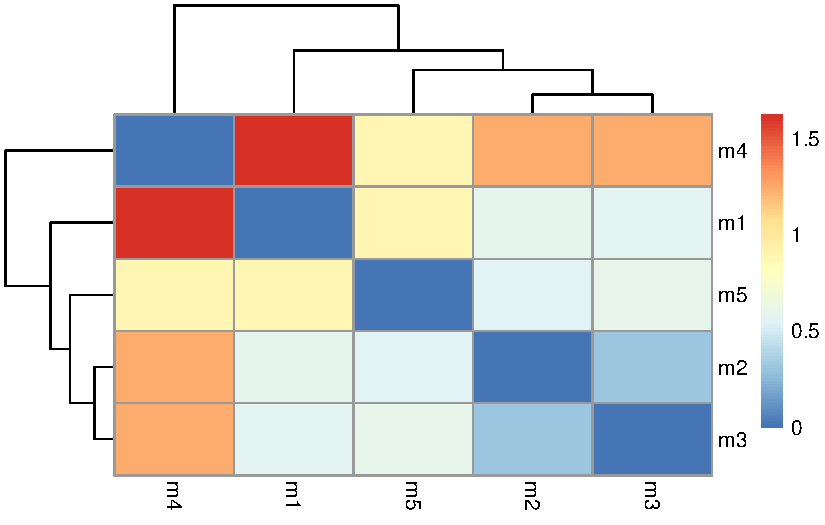
\includegraphics[keepaspectratio]{lab_files/figure-pdf/unnamed-chunk-6-1.pdf}}

\begin{Shaded}
\begin{Highlighting}[]
\CommentTok{\# Change this for YOUR results dir name}
\NormalTok{results\_dir }\OtherTok{\textless{}{-}} \StringTok{"hivprdimer\_23119/"} 
\end{Highlighting}
\end{Shaded}

\begin{Shaded}
\begin{Highlighting}[]
\CommentTok{\# File names for all PDB models}
\NormalTok{pdb\_files }\OtherTok{\textless{}{-}} \FunctionTok{list.files}\NormalTok{(}\AttributeTok{path=}\StringTok{"HIVPR\_monomer\_03c0b"}\NormalTok{,}
                        \AttributeTok{pattern=}\StringTok{"*.pdb"}\NormalTok{,}
                        \AttributeTok{full.names =} \ConstantTok{TRUE}\NormalTok{)}

\CommentTok{\# Print our PDB file names}
\FunctionTok{basename}\NormalTok{(pdb\_files)}
\end{Highlighting}
\end{Shaded}

\begin{verbatim}
[1] "HIVPR_monomer_03c0b_unrelaxed_rank_001_alphafold2_ptm_model_4_seed_000.pdb"
[2] "HIVPR_monomer_03c0b_unrelaxed_rank_002_alphafold2_ptm_model_5_seed_000.pdb"
[3] "HIVPR_monomer_03c0b_unrelaxed_rank_003_alphafold2_ptm_model_3_seed_000.pdb"
[4] "HIVPR_monomer_03c0b_unrelaxed_rank_004_alphafold2_ptm_model_2_seed_000.pdb"
[5] "HIVPR_monomer_03c0b_unrelaxed_rank_005_alphafold2_ptm_model_1_seed_000.pdb"
\end{verbatim}

\begin{Shaded}
\begin{Highlighting}[]
\FunctionTok{library}\NormalTok{(bio3d)}

\CommentTok{\# Read all data from Models }
\CommentTok{\#  and superpose/fit coords}
\NormalTok{pdbs }\OtherTok{\textless{}{-}} \FunctionTok{pdbaln}\NormalTok{(pdb\_files, }\AttributeTok{fit=}\ConstantTok{TRUE}\NormalTok{, }\AttributeTok{exefile=}\StringTok{"msa"}\NormalTok{)}
\end{Highlighting}
\end{Shaded}

\begin{verbatim}
Reading PDB files:
HIVPR_monomer_03c0b/HIVPR_monomer_03c0b_unrelaxed_rank_001_alphafold2_ptm_model_4_seed_000.pdb
HIVPR_monomer_03c0b/HIVPR_monomer_03c0b_unrelaxed_rank_002_alphafold2_ptm_model_5_seed_000.pdb
HIVPR_monomer_03c0b/HIVPR_monomer_03c0b_unrelaxed_rank_003_alphafold2_ptm_model_3_seed_000.pdb
HIVPR_monomer_03c0b/HIVPR_monomer_03c0b_unrelaxed_rank_004_alphafold2_ptm_model_2_seed_000.pdb
HIVPR_monomer_03c0b/HIVPR_monomer_03c0b_unrelaxed_rank_005_alphafold2_ptm_model_1_seed_000.pdb
.....

Extracting sequences

pdb/seq: 1   name: HIVPR_monomer_03c0b/HIVPR_monomer_03c0b_unrelaxed_rank_001_alphafold2_ptm_model_4_seed_000.pdb 
pdb/seq: 2   name: HIVPR_monomer_03c0b/HIVPR_monomer_03c0b_unrelaxed_rank_002_alphafold2_ptm_model_5_seed_000.pdb 
pdb/seq: 3   name: HIVPR_monomer_03c0b/HIVPR_monomer_03c0b_unrelaxed_rank_003_alphafold2_ptm_model_3_seed_000.pdb 
pdb/seq: 4   name: HIVPR_monomer_03c0b/HIVPR_monomer_03c0b_unrelaxed_rank_004_alphafold2_ptm_model_2_seed_000.pdb 
pdb/seq: 5   name: HIVPR_monomer_03c0b/HIVPR_monomer_03c0b_unrelaxed_rank_005_alphafold2_ptm_model_1_seed_000.pdb 
\end{verbatim}

\begin{Shaded}
\begin{Highlighting}[]
\CommentTok{\# Read a reference PDB structure}
\NormalTok{pdb }\OtherTok{\textless{}{-}} \FunctionTok{read.pdb}\NormalTok{(}\StringTok{"1hsg"}\NormalTok{)}
\end{Highlighting}
\end{Shaded}

\begin{verbatim}
  Note: Accessing on-line PDB file
\end{verbatim}

\begin{Shaded}
\begin{Highlighting}[]
\FunctionTok{plotb3}\NormalTok{(pdbs}\SpecialCharTok{$}\NormalTok{b[}\DecValTok{1}\NormalTok{,], }\AttributeTok{typ=}\StringTok{"l"}\NormalTok{, }\AttributeTok{lwd=}\DecValTok{2}\NormalTok{, }\AttributeTok{sse=}\NormalTok{pdb)}
\end{Highlighting}
\end{Shaded}

\begin{verbatim}
Warning in plotb3(pdbs$b[1, ], typ = "l", lwd = 2, sse = pdb): Length of input
'sse' does not equal the length of input 'x'; Ignoring 'sse'
\end{verbatim}

\begin{Shaded}
\begin{Highlighting}[]
\FunctionTok{points}\NormalTok{(pdbs}\SpecialCharTok{$}\NormalTok{b[}\DecValTok{2}\NormalTok{,], }\AttributeTok{typ=}\StringTok{"l"}\NormalTok{, }\AttributeTok{col=}\StringTok{"red"}\NormalTok{)}
\FunctionTok{points}\NormalTok{(pdbs}\SpecialCharTok{$}\NormalTok{b[}\DecValTok{3}\NormalTok{,], }\AttributeTok{typ=}\StringTok{"l"}\NormalTok{, }\AttributeTok{col=}\StringTok{"blue"}\NormalTok{)}
\FunctionTok{points}\NormalTok{(pdbs}\SpecialCharTok{$}\NormalTok{b[}\DecValTok{4}\NormalTok{,], }\AttributeTok{typ=}\StringTok{"l"}\NormalTok{, }\AttributeTok{col=}\StringTok{"darkgreen"}\NormalTok{)}
\FunctionTok{points}\NormalTok{(pdbs}\SpecialCharTok{$}\NormalTok{b[}\DecValTok{5}\NormalTok{,], }\AttributeTok{typ=}\StringTok{"l"}\NormalTok{, }\AttributeTok{col=}\StringTok{"orange"}\NormalTok{)}
\FunctionTok{abline}\NormalTok{(}\AttributeTok{v=}\DecValTok{100}\NormalTok{, }\AttributeTok{col=}\StringTok{"gray"}\NormalTok{)}
\end{Highlighting}
\end{Shaded}

\pandocbounded{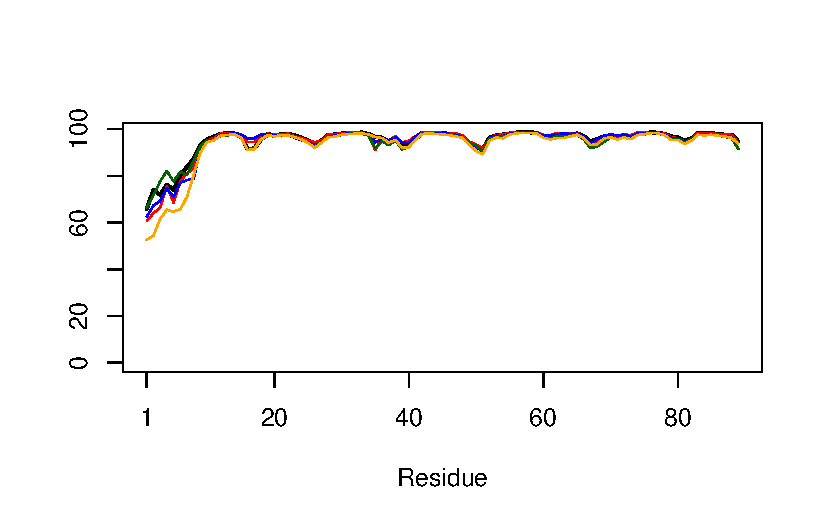
\includegraphics[keepaspectratio]{lab_files/figure-pdf/unnamed-chunk-11-1.pdf}}

\begin{Shaded}
\begin{Highlighting}[]
\NormalTok{core }\OtherTok{\textless{}{-}} \FunctionTok{core.find}\NormalTok{(pdbs)}
\end{Highlighting}
\end{Shaded}

\begin{verbatim}
 core size 88 of 89  vol = 2.858 
 core size 87 of 89  vol = 1.843 
 core size 86 of 89  vol = 0.913 
 core size 85 of 89  vol = 0.396 
 FINISHED: Min vol ( 0.5 ) reached
\end{verbatim}

\begin{Shaded}
\begin{Highlighting}[]
\NormalTok{core.inds }\OtherTok{\textless{}{-}} \FunctionTok{print}\NormalTok{(core, }\AttributeTok{vol=}\FloatTok{0.5}\NormalTok{)}
\end{Highlighting}
\end{Shaded}

\begin{verbatim}
# 86 positions (cumulative volume <= 0.5 Angstrom^3) 
  start end length
1     1   1      1
2     3   3      1
3     6  89     84
\end{verbatim}

\begin{Shaded}
\begin{Highlighting}[]
\NormalTok{xyz }\OtherTok{\textless{}{-}} \FunctionTok{pdbfit}\NormalTok{(pdbs, core.inds, }\AttributeTok{outpath=}\StringTok{"corefit\_structures"}\NormalTok{)}
\end{Highlighting}
\end{Shaded}

calculate RMSF - how far apart each amino-acid is across all 5 AlphaFold
models

\begin{Shaded}
\begin{Highlighting}[]
\NormalTok{rf }\OtherTok{\textless{}{-}} \FunctionTok{rmsf}\NormalTok{(pdbs}\SpecialCharTok{$}\NormalTok{xyz)}
\FunctionTok{plot.bio3d}\NormalTok{(rf)}
\end{Highlighting}
\end{Shaded}

\pandocbounded{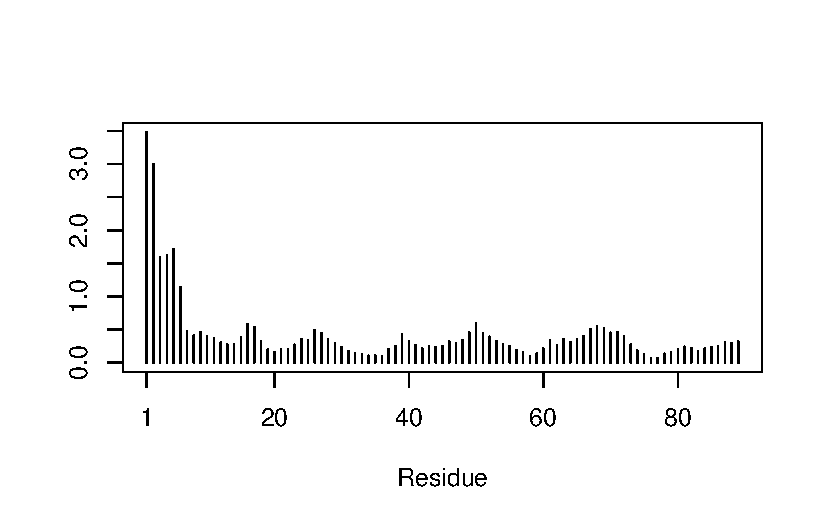
\includegraphics[keepaspectratio]{lab_files/figure-pdf/unnamed-chunk-15-1.pdf}}

\#\#2. HIV-PR Dimer

\subsubsection{RMSD}\label{rmsd}

\subsubsection{RMSF}\label{rmsf}

\subsubsection{Residue Conservation}\label{residue-conservation}

Read the AF MSA

\begin{Shaded}
\begin{Highlighting}[]
\NormalTok{aln\_file }\OtherTok{\textless{}{-}} \FunctionTok{list.files}\NormalTok{(}\AttributeTok{path=}\StringTok{"HIVPR\_monomer\_03c0b/"}\NormalTok{,}
                       \AttributeTok{pattern=}\StringTok{".a3m$"}\NormalTok{,}
                        \AttributeTok{full.names =} \ConstantTok{TRUE}\NormalTok{)}
\NormalTok{aln\_file}
\end{Highlighting}
\end{Shaded}

\begin{verbatim}
[1] "HIVPR_monomer_03c0b/HIVPR_monomer_03c0b.a3m"
\end{verbatim}

\begin{Shaded}
\begin{Highlighting}[]
\NormalTok{aln }\OtherTok{\textless{}{-}} \FunctionTok{read.fasta}\NormalTok{(aln\_file[}\DecValTok{1}\NormalTok{], }\AttributeTok{to.upper =} \ConstantTok{TRUE}\NormalTok{)}
\end{Highlighting}
\end{Shaded}

\begin{verbatim}
[1] " ** Duplicated sequence id's: 101 **"
\end{verbatim}

\begin{Shaded}
\begin{Highlighting}[]
\NormalTok{sim }\OtherTok{\textless{}{-}} \FunctionTok{conserv}\NormalTok{(aln)}
\end{Highlighting}
\end{Shaded}

Plot this conservation result

\begin{Shaded}
\begin{Highlighting}[]
\FunctionTok{plot}\NormalTok{(sim, }\AttributeTok{typ=}\StringTok{"h"}\NormalTok{)}
\end{Highlighting}
\end{Shaded}

\pandocbounded{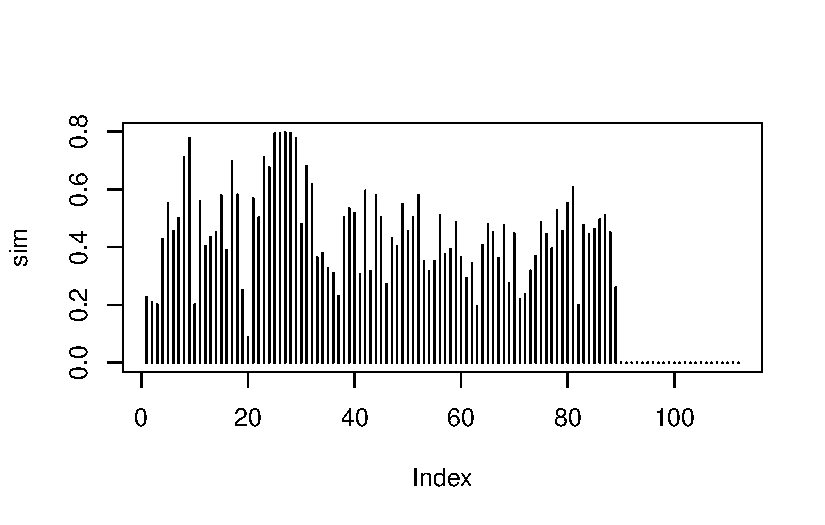
\includegraphics[keepaspectratio]{lab_files/figure-pdf/unnamed-chunk-18-1.pdf}}

\begin{Shaded}
\begin{Highlighting}[]
\NormalTok{con }\OtherTok{\textless{}{-}} \FunctionTok{consensus}\NormalTok{(aln, }\AttributeTok{cutoff =} \FloatTok{0.9}\NormalTok{)}
\NormalTok{con}\SpecialCharTok{$}\NormalTok{seq}
\end{Highlighting}
\end{Shaded}

\begin{verbatim}
  [1] "-" "-" "-" "-" "-" "-" "-" "-" "-" "-" "-" "-" "-" "-" "-" "-" "-" "-"
 [19] "-" "-" "-" "-" "-" "-" "D" "-" "G" "-" "-" "-" "-" "-" "-" "-" "-" "-"
 [37] "-" "-" "-" "-" "-" "-" "-" "-" "-" "-" "-" "-" "-" "-" "-" "-" "-" "-"
 [55] "-" "-" "-" "-" "-" "-" "-" "-" "-" "-" "-" "-" "-" "-" "-" "-" "-" "-"
 [73] "-" "-" "-" "-" "-" "-" "-" "-" "-" "-" "-" "-" "-" "-" "-" "-" "-" "-"
 [91] "-" "-" "-" "-" "-" "-" "-" "-" "-" "-" "-" "-" "-" "-" "-" "-" "-" "-"
[109] "-" "-" "-" "-"
\end{verbatim}

\^{} P .. DTGAD for 0.9 there will be D and G

\subsubsection{AF scores (pLDD \& PAE score
plots)}\label{af-scores-pldd-pae-score-plots}

The pLDDT scores are stored in the PDB models ``B-factor'' col and in a
separate JSON format file in the results directory. We can use either:

\begin{Shaded}
\begin{Highlighting}[]
\FunctionTok{plotb3}\NormalTok{(pdbs}\SpecialCharTok{$}\NormalTok{b[}\DecValTok{1}\NormalTok{,], }\AttributeTok{typ=}\StringTok{"l"}\NormalTok{, }\AttributeTok{lwd=}\DecValTok{2}\NormalTok{, }\AttributeTok{sse=}\NormalTok{pdb)}
\end{Highlighting}
\end{Shaded}

\begin{verbatim}
Warning in plotb3(pdbs$b[1, ], typ = "l", lwd = 2, sse = pdb): Length of input
'sse' does not equal the length of input 'x'; Ignoring 'sse'
\end{verbatim}

\begin{Shaded}
\begin{Highlighting}[]
\FunctionTok{points}\NormalTok{(pdbs}\SpecialCharTok{$}\NormalTok{b[}\DecValTok{2}\NormalTok{,], }\AttributeTok{typ=}\StringTok{"l"}\NormalTok{, }\AttributeTok{col=}\StringTok{"red"}\NormalTok{)}
\FunctionTok{points}\NormalTok{(pdbs}\SpecialCharTok{$}\NormalTok{b[}\DecValTok{3}\NormalTok{,], }\AttributeTok{typ=}\StringTok{"l"}\NormalTok{, }\AttributeTok{col=}\StringTok{"blue"}\NormalTok{)}
\FunctionTok{points}\NormalTok{(pdbs}\SpecialCharTok{$}\NormalTok{b[}\DecValTok{4}\NormalTok{,], }\AttributeTok{typ=}\StringTok{"l"}\NormalTok{, }\AttributeTok{col=}\StringTok{"darkgreen"}\NormalTok{)}
\FunctionTok{points}\NormalTok{(pdbs}\SpecialCharTok{$}\NormalTok{b[}\DecValTok{5}\NormalTok{,], }\AttributeTok{typ=}\StringTok{"l"}\NormalTok{, }\AttributeTok{col=}\StringTok{"orange"}\NormalTok{)}
\end{Highlighting}
\end{Shaded}

\pandocbounded{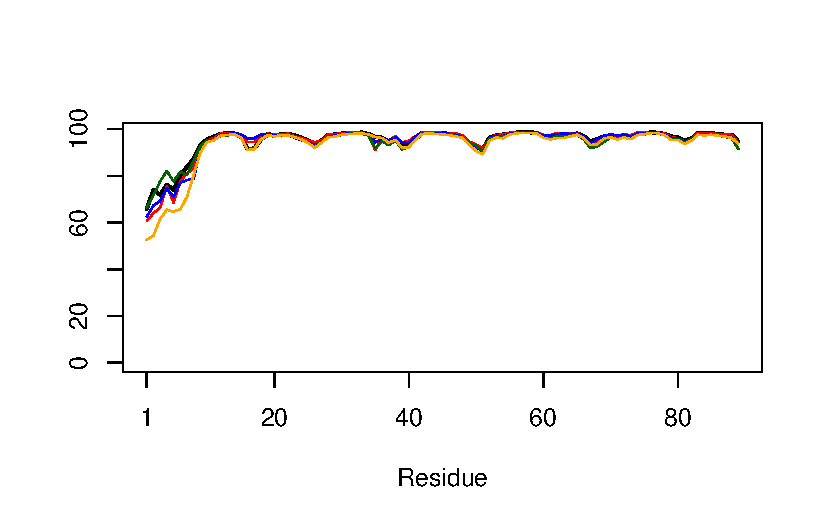
\includegraphics[keepaspectratio]{lab_files/figure-pdf/unnamed-chunk-20-1.pdf}}

\begin{Shaded}
\begin{Highlighting}[]
\CommentTok{\#plot(m1.pdb$atom$b[m1.pdb$calpha], typ ="h")}
\end{Highlighting}
\end{Shaded}

\subsubsection{pLDDT \& PAE score plots}\label{plddt-pae-score-plots}

\subsection{3. My Find-A-Gene Sequence}\label{my-find-a-gene-sequence}

MHSKKYKNLCKLCMNDCSRTHKNPYYDYSGALKCLEEAGDVGFMKHTTVPDSEKSKYELLCKNGTRKSVNDFATCHLAKVPAHAVVSRKDADLANRIWDMLQIAMKFSLFSSTNYKAKDLLFRDSTAKLVQIPKGTDSFLYLGAEYMSIVHSLQKAGPDIKRDAKEVKWCAVGQEETKKCDNWALSIHADSGKDKISWDNAPTVDDCIKKIMRKEADAMTLDGGELYTAGMCGLVPVMAEQYDEAKCSESGDTAASSYYAVAVVKNGTGFSWADLRGKKSCHTGMGRTAGWNVPMGLIHRDTNDCEFSKFFSESCAPGADEGSSLCKLCKGKDNVGVRKCKASTEELYYSYAGAFRCLVEGGGDVAFVKHTTVRENSDGNGPSWASALKSADFELLCLDNTTAPISQHLKCHLAKVPAHAVVTRPEMRDQVVAVLKDQESLFGNNGSDTGLFTMFQSKEGSNLLFKDSTKCLQEVIKGQSFKDFLGKEYYDAVTSLRQCSTSASELEKACTFHTCQQKV

\subsubsection{Read AF Models}\label{read-af-models}

\subsubsection{RMSD}\label{rmsd-1}

\subsubsection{RMSF}\label{rmsf-1}

\subsubsection{Residue Conservation}\label{residue-conservation-1}

\subsubsection{AF scores (pLDDT \& PAE score
plots)}\label{af-scores-plddt-pae-score-plots}




\end{document}
